% !TeX program = xelatex

\chapter{Nutzerstudie}
\label{cha:Usability_study}

\section{Inhalte der Studie}
\label{sec:study_content}
Um eine Aussage über die Nutzbarkeit der Anwendung zu treffen, wurden zwei Verschiedene Studien durchgeführt.
Die erste Studie nutzt eine Thinking Aloud Technik, bei der die Probanden unter einer vorgegebenen Aufgabenstellung die Anwendung verwenden und dabei ihre Gedanken laut äußern.
Es wird dabei nicht nur die Aufgabe bewertet, sondern auch die wie die Nutzer Anwendung selbst warnehmen, welche Probleme sie haben und wie sie diese lösen und ob sie die Anwendung intuitiv bedienen können.
Dadurch kann im Nachhinein eine Aussage getroffen werden inwieweit die erstellten Konzepte vom Nutzer angenommen werden und ob sie so intuitiv bedienbar sind, wie angenommen.
Gerade im Bezug auf Shneidermans Golden Rules \cite{10.5555/3033040} lässt sich dies bewerten.

Die zweite Studie ist etwas größer angelegt und soll die Anwendung in einem größeren Rahmen bewerten. Hierzu wurden die Nutzer in zwei Gruppen aufgeteilt und bekommen jeweils eine leicht abgewandelte Aufgabe gestellt.
Diese können sie alleine lösen um anschliesend ihre Erfahrungen und Meinungen in einem Fragebogen zu äußern.
Der Fragebogen ist in drei Teile aufgeteilt. Im ersten Abschnitt werden die Nutzer gebeten, die Anwendung zu bewerten und ihre Erfahrungen zu äußern. Dies wird mit Hilfe des System Usability Scale (SUS) Fragebogens \cite{brooke1996sus} durchgeführt. 
Im zweiten Teil wird die mentale Leistung der Nutzer gemessen und dafür der Nasa Task Load Index (NASA-TLX) \cite{HART1988139} verwendet.
Um die in den ersten beiden Teilen in einen Kontext zu setzen, werden im dritten Teil noch einige Fragen zur Person und dem Umgang mit der Anwendung gestellt.

Der NASA-TLX Frageboge existiert seit 1988, ist anerkannt und weit verbreitet. Ziel des Fragebogens ist es zu messen, wie mental Fordernd die Anwendung ist. 
Mithilfe von 6 Fragen wird die mentale Belastung in den 6 folgenden Kategorien bewertet:
\begin{description}
    \item[Geistige Anforderung] Wie geistig anspruchsvoll war die Aufgabe?
    \item[Körperliche Anforderung] Wie körperlich anspruchsvoll war die Aufgabe?
    \item[Zeitliche Anforderung] Wie gehetzt oder eilig war das Tempo der Aufgabe?
    \item[Leistung] Wie erfolgreich waren Sie bei der Erledigung dessen, was von Ihnen verlangt wurde?
    \item[Anstrengung] Wie hart mussten Sie arbeiten, um Ihre Leistung zu erreichen?
    \item[Frustration] Wie unsicher, entmutigt, gereizt, gestresst und genervt waren Sie?
\end{description}

Die Bewertung erfolgt auf einer Skala von 1 bis 10, wobei 0 für sehr geringe Anforderung steht und 10 für sehr hohe Anforderung. Aufsummiert ergibt der finale Wert die mentale Anforderung. Ist der Wert hoch, dann muss der Nutzer sich stark auf die Anwendung konzentrieren. 
Bei einem geringen Wert hat der Nutzer wenig Probleme mit der Anwendung klar zu kommen.

Der System Usability Scale Fragebogen ist ebenfalls sehr weit verbreitet und wird seit 1986 verwendet. Er besteht aus 10 Fragen (Siehe \ref{itm:sus_questions}), die in einer 5-Punkte Likert-Skala bewertet werden. Eine 5 steht dabei für "Stimme voll zu" und eine 1 für "Stimme überhaupt nicht zu". Die Fragen sind im wechsel 
positiv und negativ formuliert, um eine Verzerrung der Ergebnisse zu verhindern. Dies macht die Auswertung ein wenig komplizierter, da die negativ formulierten Fragen umgerechnet werden müssen. Nach einer Normalisierung werden die negativen Werte umgerechnet und danach aufsummiert und mit 2.5 multipliziert.

Die Fragen sind:

\begin{itemize}
\label{itm:sus_questions}
    \item Ich denke, ich würde die Website/die App regelmäßig nutzen.
    \item Die Website/die App scheint mir unnötig kompliziert zu sein.
    \item Ich finde, die Website/die App ist einfach zu bedienen.
    \item Ich denke, ich würde technische Unterstützung benötigen, um die Website/die App nutzen zu können.
    \item Ich denke, dass die verschiedenen Funktionen der Website/des Apps gut integriert sind.
    \item Die Website/die App scheint mir zu inkonsistent.
    \item Ich glaube, dass die meisten Menschen schnell lernen können, wie man die Website/die App benutzt.
    \item Die Website/die App scheint sehr umständlich in der Nutzung zu sein.
    \item Ich fühle mich sehr sicher bei der Nutzung der Website/des Apps
    \item Ich musste viel lernen, um mich mit der Website/dem App zurechtzufinden.
\end{itemize}


\section{Studienablauf}
\label{sec:study_process}
Die für dieses Projekt gewählten Personas sind divers. Sie haben einen gewissen technischen Hintergrund, sind aber keine Experten. 
Dies erlaubt daher auch eine breite Auswahl an Teilnehmern in die Studie einzubeziehen.
Für die Studie wurden 11 Probanden ausgewählt. Die Auswahl erfolgte über persönliche Kontakte, weitere Nutzer haben die Software ausgetested, aber nicht an der Studie teilgenommen.

Schaut man sich die Hintergründe der Probanden an, so fällt auf, dass diese sehr unterschiedlich sind. Die Probanden sind zwischen 24 und 40 Jahre alt, sind in unterschiedlichen, auch nicht technischen Berufen tätig und zeigen eine ziemlich unterschiedliche technische Grundfähigkeit auf.
Es gibt bereits Teilnehmer mit einem geringen Vorwissen im Bereich der Simulationssoftware.

Da es, wie in der im Anhang beigefügten Aufgabenstellung zwei unterschiedliche Aufgaben gibt, wurden die Probanden in zwei Gruppen aufgeteilt, welche aus jeweils 5 Teilnehmern bestanden.
Teilnehmer Nr. 11 hatte beide Aufgaben durchgeführt. 
Mit außnahme einiger weniger Probanden, welche zusätzlich noch eine kurzen Thinking Aloud Technik unterzogen wurden, durften die meisten Probanen sich selber ohne weitere Unterstützung an der Aufgabe versuchen.
Da die Webanwendung auf einem Server läuft, mussten die Probanden nicht extra eine Anwendung installieren, sondern konnten diese direkt über den Browser aufrufen. Aufgabenstellung und Testdaten wurden den Probanden in einer Datei zur Verfügung gestellt.

Teilnehmer der Thinking Aloud Studie bekamen die gleiche Aufgabe gestellt, diese sollten sie aber unter überwachung durchführen und wurden gebeten, ihre Gedanken während der Aufgabenlösung laut auszusprechen. Diese, sowie ihre Interaktionen, wurden alle protokolliert.
Wichtig ist, dass die Probanden dabei nicht beeinflusst wurden und somit die Aufgabe frei und selbstständig lösen mussten.
Die Protokolle erlauben einen Einblick in die Gedanken der Nutzer und erlauben Rückschlüsse darüber, inwieweit der Nutzer die Prozesse und Möglichkeiten der Anwendung realisiert und versteht.



\section{Auswertung der Studie}
\subsection{Ergebnisse der Thinking Aloud Studie}
Die Studie wurde mit fünf Probanden durchgeführt, die aufgefordert wurden, die Aufgaben zu lösen und dabei ihre Gedanken laut auszusprechen, wie bereits in Sektion \ref*{sec:study_content} beschrieben.

Zu Beginn erhielten die Teilnehmer etwas Zeit, um sich mit der Software vertraut zu machen, da sie zuvor noch keine Erfahrungen mit dieser hatten. Dieser Schritt war entscheidend, um ihnen ein grundlegendes 
Verständnis für die Funktionsweise der Software zu vermitteln.

Während der Aufgabenbearbeitung hatten die Teilnehmer im Allgemeinen wenig Schwierigkeiten. Die meisten verstanden die Aufgabenstellung schnell und konnten durch das Durchsuchen der Menüs die benötigten Funktionen finden. 
Oft wichen sie anfangs von der eigentlichen Aufgabe ab und erforschten eigenständig die Möglichkeiten der Software. Positiv hervorgehoben wurden dabei die integrierten Tooltips.

Bei der Definition der Generierung synthetischer Daten kamen die meisten Teilnehmer gut mit dem Dialog zurecht. Der dritte Schritt, die Definition der Datenvorverarbeitung, stellte sich jedoch als verwirrend heraus. 
Die Teilnehmer waren sich über die Bedeutung der einzelnen Optionen und deren Auswirkungen auf die Daten unsicher. Hinzu kam, dass das verwendete Schema zwar eine Beschreibung für alle Optionen bot, die eingesetzte rsjf-Bibliothek jedoch 
keine Erklärungen für die Auswahl der Imputationsalgorithmen bei den Radio Buttons zur Verfügung stellte. Drei der Nutzer entdeckten zudem nicht die Möglichkeit, sich einen Graphen der Daten anzeigen zu lassen, obwohl dieser 
direkt unter der Konfiguration zu finden war. Der Teilnehmer, der den Graphen entdeckte, war sich jedoch nicht bewusst, dass man einzelne Graphen dynamisch ausblenden kann, und konnte daher nur wenig Nutzen aus der Visualisierung ziehen.

Nach dem Absenden der Konfiguration hatten die Teilnehmer wenig Schwierigkeiten, entweder testweise die Graphen zu verschieben und zu speichern oder das Training der Modelle zu starten. Besonders positiv wurde die 
prozentuale Statusanzeige während des Trainings der Modelle aufgenommen. Bei der Erstellung der Projekte hatte ein Teilnehmer bereits an der Nutzerstudie der ursprünglichen Anwendung teilgenommen und verfügte daher über 
einen guten Überblick über die notwendigen Schritte. Die anderen Teilnehmer hatten jedoch Schwierigkeiten, die Unterscheidung zwischen Projekten, Tracks und Datasets zu verstehen. Da diese Struktur jedoch zweckmäßig ist 
und einen bestimmten Nutzen verfolgt, könnten zukünftige Einarbeitungen diese Probleme beheben.

Auffällig war, dass viele Teilnehmer den Informationsbutton nicht näher betrachteten. Dieser bietet eine Visualisierung der Websockets, also der trainierenden Modelle und der gesendeten Projekte. Die Personen, die ihn 
benutzten, waren verwirrt, als sie keine Aktivität sahen, weil gerade nichts trainiert wurde. Hier ist also weitere Arbeit nötig, um die Nutzer besser über die Bedeutung und Funktion dieser Anzeige zu informieren.

\subsection{Auswertung der Fragebögen}
\label{sec:results_of_user_experience}
Die Fragebögen wurden von allen Teilnehmern ausgefüllt, einschließlich jener, die an der Thinking Aloud Technik teilnahmen. Die einzelnen Ergebnisse sind in der Tabelle \ref{tab:probanden} im Anhang dargestellt. 
Generell lässt sich sagen, dass die Nutzer die Anwendung als gut bedienbar empfanden. Die durchschnittlichen Ergebnisse auf der SUS-Skala lagen bei 76.32, was darauf hindeutet, dass die Anwendung als 
benutzerfreundlich wahrgenommen wurde. Mental fühlten sich die Nutzer nicht stark gefordert, was sich in einem durchschnittlichen TLX-Wert von 36.5 widerspiegelt, ein Indikator dafür, dass die Aufgaben ohne große Anstrengungen gelöst werden konnten.

Besonders interessant ist der Vergleich der Ergebnisse der Fragebögen im Zusammenhang mit Alter und technischer Begabung der Teilnehmer (siehe Abbildung \ref{fig:3dplot_tlx_sus}). Hierbei zeigte sich, 
dass Teilnehmer mit geringerer technischer Begabung die Anwendung weniger fordernd fanden, während jene mit durchschnittlicher Begabung dies als anspruchsvoller empfanden. Teilnehmer mit hoher technischer 
Begabung fanden die Aufgaben wiederum leichter. Dies mag zunächst kontraintuitiv erscheinen, aber unter Berücksichtigung der Beobachtungen aus der Thinking Aloud Studie ergibt sich ein schlüssiges Bild: Nutzer mit geringer technischer Begabung gingen erstaunlich schnell durch die Anwendung und klickten die meisten Funktionen direkt an, ohne sich zunächst auf die Aufgabe zu konzentrieren. Bei Nutzern mit durchschnittlichem technischen Verständnis war dies nicht der Fall; sie verhielten sich deutlich zögerlicher.

\begin{figure}[h]
    \centering
    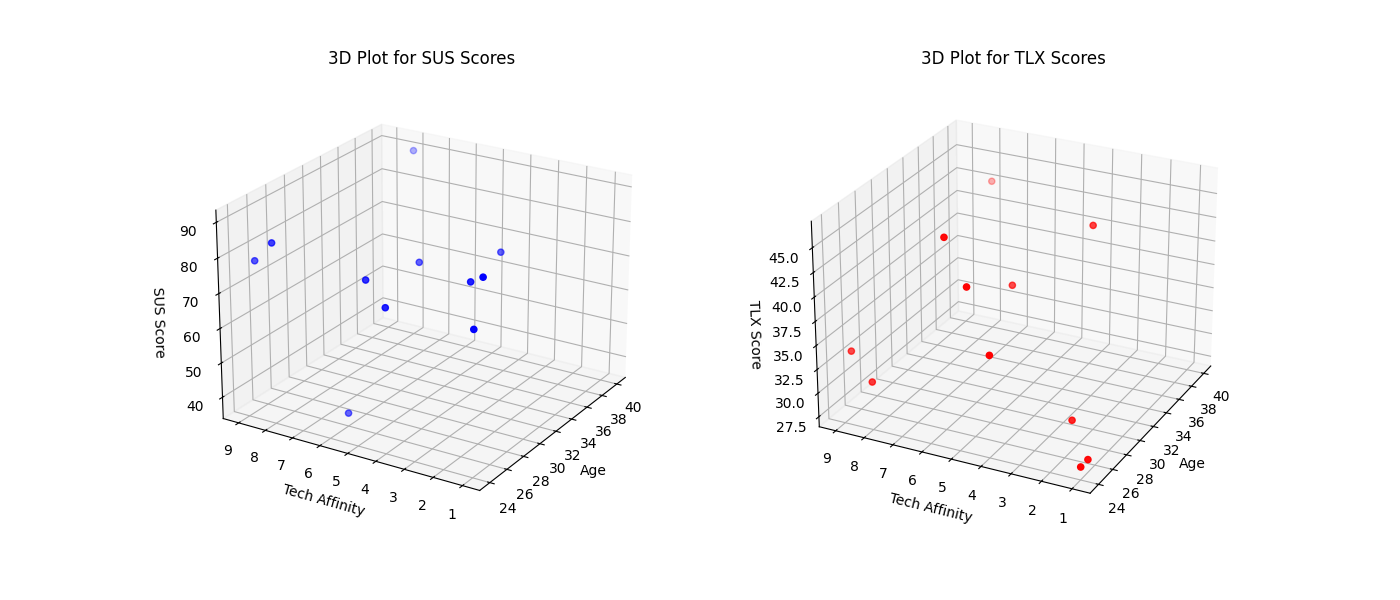
\includegraphics[width=\textwidth]{includes/figures/study/3dplot.png}
    \caption{Grafische Darstellung der Ergebnisse des NASA-TLX und SUS-Fragebogens in Abhängigkeit des Alters und der technischen Begabung}
\label{fig:3dplot_tlx_sus}
\end{figure}

Eine Korrelation des Alters mit dem Testergebnis war nicht erkennbar. Die Altersverteilung war jedoch zu klein, um aussagekräftige Schlussfolgerungen zu ziehen, insbesondere im Hinblick auf die technische 
Begabung. Während sich die technische Begabung bei den Teilnehmern in den mittleren Zwanzigern noch recht gut verteilte, war sie bei den älteren Teilnehmern deutlich höher.

Wie in Abbildung \ref{fig:study_sus} dargestellt, war insbesondere bei Frage 1, \textit{'Ich denke, ich würde die Website/die App regelmäßig nutzen.'}, eine hohe Zustimmung zu verzeichnen. Die Nutzer wurden 
gebeten, sich in die Situation zu versetzen, solch eine Software zu benötigen. Obwohl die meisten Teilnehmer in einer solchen Situation nicht sind, war es notwendig um über den Fragebogen eine valide Aussage zu erhalten.

\begin{figure}[ht]
    \centering
    \begin{minipage}{0.5\textwidth}
        \centering
        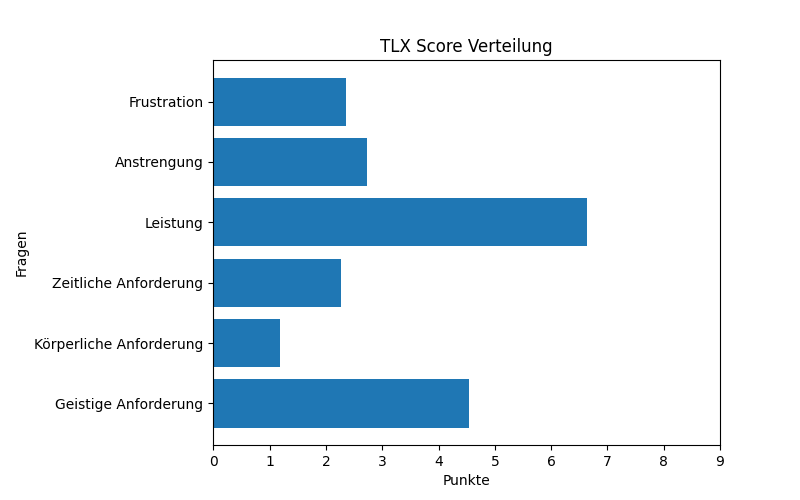
\includegraphics[width=\textwidth]{includes/figures/study/tlx.png}
        \caption{Auswertung des NASA-TLX Fragebogens}
        \label{fig:study_tlx}
    \end{minipage}\hfill
    \begin{minipage}{0.5\textwidth}
        \centering
        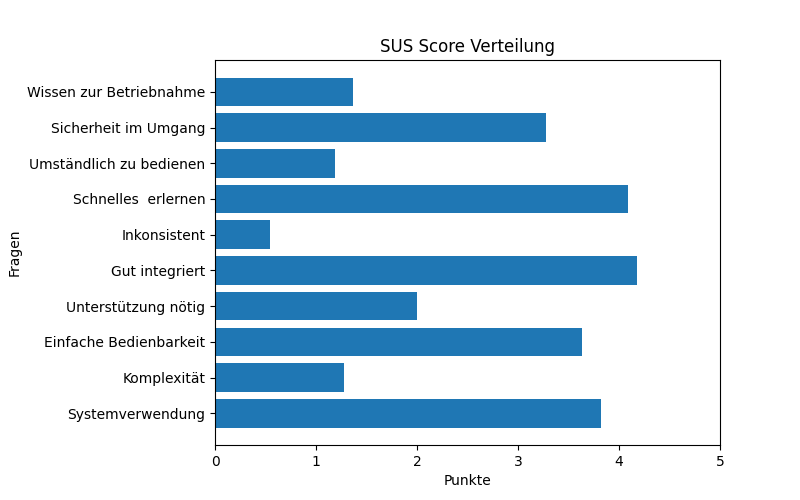
\includegraphics[width=\textwidth]{includes/figures/study/sus.png}
        \caption{Auswertung des SUS Fragebogens}
        \label{fig:study_sus}
    \end{minipage}
\end{figure}

